\documentclass[11pt]{article}

% ------------------------------------------------------------
% Packages
% ------------------------------------------------------------
\usepackage[a4paper,top=1.25in,bottom=1.8in,left=1in,right=1in]{geometry}
\usepackage{amsmath,amssymb,amsfonts}
\usepackage{xcolor}
\usepackage{graphicx}
\usepackage{tikz}
\usetikzlibrary{arrows.meta,calc,positioning}
\usepackage[hidelinks]{hyperref}
\usepackage{fancyhdr}

% ------------------------------------------------------------
% Brand colours (deep teal + burnt orange)
% ------------------------------------------------------------
\definecolor{QFTeal}{RGB}{0,92,89}
\definecolor{QFOrange}{RGB}{191,97,0}

\hypersetup{
  colorlinks=true,
  urlcolor=QFTeal,
  linkcolor=QFTeal
}

% ------------------------------------------------------------
% Header / Footer branding
% ------------------------------------------------------------
\setlength{\headheight}{95pt}  % room for big logo
\setlength{\footskip}{55pt}    % ensure footer is visible
\pagestyle{fancy}
\fancyhf{}

% Bigger logo (top-right)
\fancyhead[R]{\includegraphics[height=75pt]{qf-logo.png}}

% Branded footer (bottom-centre)
\fancyfoot[C]{%
  \footnotesize\href{https://quantumformalism.academy/}{\textcolor{QFTeal}{quantumformalism.academy}}%
}

\renewcommand{\headrulewidth}{0pt}
\renewcommand{\footrulewidth}{0pt}

% ------------------------------------------------------------
% TikZ styles (force fully solid strokes)
% ------------------------------------------------------------
\tikzset{
  qfteal/.style   ={draw=QFTeal,   line width=1.8pt, solid, draw opacity=1},
  qforange/.style ={draw=QFOrange, line width=1.8pt, solid, draw opacity=1},
}

\begin{document}
\thispagestyle{fancy} % force fancy on this page no matter what

% Slightly scale down to guarantee footer space on A4 in all viewers
\begin{center}
\begin{tikzpicture}[
  x=1cm,y=1cm,
  >=Stealth,
  line cap=round,
  line join=round,
  scale=0.88,
  transform shape
]

% --- Frame ---------------------------------------------------------------
\draw[line width=1.2pt] (-0.6,-3.8) rectangle (13.2,3.8);

% --- Left: cylinder X x [0,1] -------------------------------------------
\fill[gray!20] (1.4,-2.2) rectangle (3.6,1.6);

\fill[white] (2.5,1.6) ellipse (1.1 and 0.35);
\fill[white] (2.5,-2.2) ellipse (1.1 and 0.35);

\draw[line width=1pt] (1.4,-2.2) -- (1.4,1.6);
\draw[line width=1pt] (3.6,-2.2) -- (3.6,1.6);
\draw[line width=1pt] (2.5,1.6) ellipse (1.1 and 0.35);
\draw[line width=1pt] (2.5,-2.2) ellipse (1.1 and 0.35);

% coloured rims (solid)
\draw[qfteal]   (2.5,1.6) ellipse (1.1 and 0.35);
\draw[qforange] (2.5,-2.2) ellipse (1.1 and 0.35);

\node[anchor=east] at (1.2,1.55) {$X\times\{1\}$};
\node[anchor=east] at (1.2,-2.25) {$X\times\{0\}$};

% --- Middle arrow: h -----------------------------------------------------
\draw[->, line width=1.2pt]
  (3.8,-0.35) .. controls (5.0,-0.5) and (6.5,-0.4) .. (8.0,-0.2)
  node[midway, above=2pt] {$h$};

% --- Maps g and f --------------------------------------------------------
\draw[->, qfteal]
  (3.8,1.8) .. controls (4.8,2.7) and (6.0,2.6) .. (7.1,2.1)
  node[midway, above=2pt] {$g$};

\draw[->, qforange]
  (3.5,-2.5) .. controls (5.0,-3.1) and (6.5,-2.8) .. (7.6,-2.0)
  node[midway, below=2pt] {$f$};

% --- Right: Homotopy Surface in R^3 --------------------------------------
% Fill + draw the surface with the SAME colour to eliminate PDF hairline seams.
\path[fill=gray!30, draw=gray!30, line width=0.6pt]
  (7.5,2.0)
  .. controls (7.5,2.5) and (8.5,2.2) .. (9.3,2.4)
  .. controls (10.1,2.6) and (11.1,2.8) .. (11.1,2.3)
  .. controls (10.3, 1.0) and (10.4, -0.5) .. (11.2,-2.1)
  .. controls (11.2,-2.6) and (10.0,-2.6) .. (9.5,-1.9)
  .. controls (9.0,-2.3) and (7.8,-2.3) .. (7.8,-1.8)
  .. controls (8.6, -0.5) and (8.3, 1.0) .. (7.5,2.0)
  -- cycle;

% R^3 Axes
\draw[line width=1.8pt] (9.4,-0.1) -- (9.4,3.5);
\draw[line width=1.8pt] (9.4,-0.1) -- (6.6,-1.5);
\draw[line width=1.8pt] (9.4,-0.1) -- (12.0,-1.8);
\node[anchor=west, font=\Large] at (11.5,1.2) {$\mathbb{R}^3$};

% Top loop (g image) - force solid
\draw[qfteal]
  (7.5,2.0)
  .. controls (7.5,1.5) and (8.5,1.7) .. (9.3,1.9)
  .. controls (10.1,2.1) and (11.1,1.8) .. (11.1,2.3)
  .. controls (11.1,2.8) and (10.1,2.6) .. (9.3,2.4)
  .. controls (8.5,2.2) and (7.5,2.5) .. (7.5,2.0);

% Bottom loop (f image) - force solid
\draw[qforange]
  (7.8,-1.8)
  .. controls (7.8,-2.3) and (9.0,-2.3) .. (9.5,-1.9)
  .. controls (10.0,-1.5) and (11.2,-1.5) .. (11.2,-2.1)
  .. controls (11.2,-2.6) and (10.0,-2.6) .. (9.5,-1.9)
  .. controls (9.0,-1.2) and (7.8,-1.3) .. (7.8,-1.8);

\end{tikzpicture}
\end{center}

\end{document}